%%%%%%%%%%%%%%%%%%%%%%%%%%%%%%%%%%%%%%%%%
% Doctoral Proposal
% LaTeX Template
% Version 1.0 (25/10/18)
%
% Author: Fred Guth (fredguth@fredguth.com
%
% License:
% CC BY-NC-SA 3.0 (http://creativecommons.org/licenses/by-nc-sa/3.0/)
%
%%%%%%%%%%%%%%%%%%%%%%%%%%%%%%%%%%%%%%%%%

%----------------------------------------------------------------------------------------
%	PACKAGES AND OTHER DOCUMENT CONFIGURATIONS
%----------------------------------------------------------------------------------------

\documentclass[
12pt, % Default font size is 10pt, can alternatively be 11pt or 12pt
a4paper, % Alternatively letterpaper for US letter
onecolumn, % Alternatively twocolumn
% portrait % Alternatively landscape
]{article}

%%%%%%%%%%%%%%%%%%%%%%%%%%%%%%%%%%%%%%%%%
% Paper Notes
% Structure Specification File
% Version 1.0 (25/10/18)
%
% Author: Fred Guth (fredguth@fredguth.com
%
% License:
% CC BY-NC-SA 3.0 (http://creativecommons.org/licenses/by-nc-sa/3.0/)
%
%%%%%%%%%%%%%%%%%%%%%%%%%%%%%%%%%%%%%%%%%%%%%%%%%%%%%%%%%%%%%%%%%%%%%%%%%%%%%%%%%%

%----------------------------------------------------------------------------------------
%	REQUIRED PACKAGES
%----------------------------------------------------------------------------------------

\usepackage[includeheadfoot,columnsep=2cm, left=1in, right=1in, top=.5in, bottom=.5in]{geometry} % Margins
\usepackage[para]{footmisc}
\usepackage[utf8]{inputenc}
% \usepackage{XCharter} % XCharter as the main font
\usepackage{times}
\usepackage{booktabs}
% \usepackage{natbib} % Use natbib to manage the reference
\usepackage{bibentry}
\usepackage{blindtext}
\usepackage[inline]{enumitem}
\nobibliography*
\bibliographystyle{unsrt} % Citation style
\usepackage{setspace}
\usepackage[brazil]{babel} % Use english by default
\usepackage{pdfpages}

%----------------------------------------------------------------------------------------
%	CUSTOM COMMANDS
%----------------------------------------------------------------------------------------

\newcommand{\doctitle}[1]{\renewcommand{\doctitle}{#1}} % Define a command for storing the proposal title

\newcommand{\horrule}[1]{\rule{\linewidth}{#1}} % Create
\newcommand{\datenotesstarted}[1]{\renewcommand{\datenotesstarted}{#1}} % Define a command to store the date when notes were first made
\newcommand{\docdate}[1]{\renewcommand{\docdate}{#1}} % Define a command to store the date line in the title

\newcommand{\docauthor}[1]{\renewcommand{\docauthor}{#1}} % Define a command for storing the article notes author
\newcommand{\authorid}[1]{\renewcommand{\authorid}{#1}} % Define a command for storing the author id
\setlist[description]{font=\normalfont}

% Define a command for the structure of the document cover page
\newcommand{\printcover}{
\pagenumbering{gobble}


\begin{center}

  \bigskip

  PROGRAMA DE PÓS-GRADUAÇÃO EM INFORMÁTICA

  \bigskip
  \bigskip
  \bigskip
  \bigskip
\end{center}


\begin{description}[align=left,labelwidth=5cm]
  
    \item[Nome:] \docauthor
    
    \item[CPF:] \authorid
  
\end{description}
  

  \bigskip
  \bigskip
  
\textbf{Proposta de Projeto de Pesquisa}
  \bigskip
  \bigskip

  
\begin{description}[align=left,labelwidth=5cm]
  
    \item[Título:] \doctitle
    \bigskip
    \bigskip
    \bigskip
    \bigskip
    \item[Linha de Pesquisa:] Sistemas de Computação
    
    \item[Área de Pesquisa:] Visão Computacional
  
\end{description}

\newpage


}

%----------------------------------------------------------------------------------------
%	STRUCTURE MODIFICATIONS
%----------------------------------------------------------------------------------------

\setlength{\parskip}{3pt} % Slightly increase spacing between paragraphs

% Uncomment to center section titles
%\usepackage{sectsty}
%\sectionfont{\centering}

% Uncomment for Roman numerals for section numbers
%\renewcommand\thesection{\Roman{section}}
 % Input the file specifying the document layout and structure

%----------------------------------------------------------------------------------------
%	ARTICLE INFORMATION
%----------------------------------------------------------------------------------------

\doctitle{Transferência de Aprendizado em Visão Computacional} % The title of the proposal

\datenotesstarted{\today} % The date when these notes were first made
\docdate{\datenotesstarted; rev. \today} % The date when the notes were lasted updated (automatically the current date)

\docauthor{Frederico Guth} % Your name
\authorid{273.723.818-86}
%----------------------------------------------------------------------------------------

\begin{document}

\pagestyle{myheadings} % Use custom headers
\markright{Transferência de Aprendizado em Visão Computacional} % Place the article information into the header

%----------------------------------------------------------------------------------------
%	PRINT ARTICLE INFORMATION
%----------------------------------------------------------------------------------------

\thispagestyle{plain} % Plain formatting on the first page

\printcover % Print the title

% \begin{center}

%   \horrule{0.5pt} \\[0.4cm] % Thin top horizontal rule

%   \bigskip

%   \textbf{\Large{\doctitle}}
  
%   \bigskip
  
%   \docauthor

%   \bigskip
  

%   \horrule{2pt} \\[0.5cm] % Thick bottom horizontal rule

% \end{center}

%----------------------------------------------------------------------------------------
%	ARTICLE NOTES
%----------------------------------------------------------------------------------------
\thispagestyle{plain}
\setlist[description]{font=\bfseries}
\setcounter{page}{2}
\pagenumbering{arabic}
\onehalfspacing

%------------------------------------------------
\section{Introdução}

Recentes avanços na área de Visão Computacional tornam possíveis aplicações que são capazes de reconher pessoas, lugares e objetos com acurácia super-humana \cite{fei}, diagnosticar câncer de pele tão bem quanto dermatologistas \cite{skin_cancer_doi:10.1093/annonc/mdy166},  ver através de paredes usando sinais de rádio \cite{wifi}, entre tantas outras. 


Neste contexto, é compreensível se iludir com o sensacionalismo e até pensar que Aprendizado Profundo (DL\footnote{Deep Learning}) seja uma área "resolvida" \textemdash longe disso. Os melhores casos de sucesso foram desenvolvidos exclusivamente para uma tarefa, em um único domínio; sobre a premissa básica que os dados com os quais o modelo será testado são do mesmo espaço de características e possuem a mesma distribuição que os dados de treinamento \cite{Pan}. Em outras palavras, temos algoritmos cada vez melhores em encontrar padrões em uma grande quantidade de dados rotulados, mas ainda deficientes na capacidade de generalizar para condições diferentes daquelas encontradas no treinamento. 

% Ao mesmo tempo que bancos de imagens de larga escala são um dos componentes chave para progresso obtido nos últimos anos, cada vez mais a necessidade de dados são um fator limitante para aplicações práticas.  Uma quantidade importante de comportamentos da natureza e atividades humanas obedecem a uma distribuição de cauda longa, o que torna bastante difícil a coleta representativa de dados. Há também o  alto custo de rotulação: em diversas áreas de aplicação, e.g. na medicina, dados bem rotulados são extremamente difíceis e levam anos para serem obtidos em pequena quantidade. 

Transferência de Aprendizado (TL\footnote{Transfer Learning}) é a área que pesquisa como armazenar conhecimento adquirido em um domínio ou tarefa e aplicá-lo a um novo problema. Essa capacidade permite lidar com a insuficiência de dados rotulados e é absolutamente necessária para o uso de inteligência artificial em larga escala que vai além das tarefas e domínios para os quais a disponibilidade de dados rotulados é ambundante. Em outras palavras, apesar de todo o sucesso, os modelos atuais atacam apenas os casos fáceis em termos de disponibilidade de dados. Para lidar com a variabilidade cauda longa do mundo, precisamos aprender a tranferir aprendizado.

% \subsection{Definição Formal}
% Transferência de Aprendizado envolve os conceitos de \textit{domínio} e \textit{tarefa}. Seguindo a notação de \cite{Pan}, um domínio $\mathcal{D}$ é composto de um espaço de características $\mathcal{X}\subset R^d$ e uma distribuição marginal $P(\mathrm{X})$, onde $\mathrm{X}=\{x_1, \dots, x_n\}\in\mathcal{X} $. Para um problema de classificação de imagens, por exemplo, $\mathcal{X}$ é o espaço de todas possíveis representações de imagens, com suas dimensões e canais, $x_i$ é uma imagem e $X$ é o \textit{dataset} de treinamento. 

% Dado um domínio $\mathcal{D}=\{\mathcal{X}, P(X)\}$, uma tarefa $\mathcal{T}$ é definida pelo espaço de rótulos $\mathcal{Y}$ com distribuição condicional $P(\mathrm{Y}|\mathrm{X})$, ou seja, $\mathcal{T}=\{\mathcal{Y}, f(\cdot)\}$, onde $f(\cdot)$ é uma função objetivo que dado um $x_i \in \mathcal{D}$, prediz seu correspondente $y_i \in \mathcal{Y}$. 

% Dado um domínio fonte $\mathcal{D_S}$ e uma tarefa $\mathcal{T_S}$, um domínio destino $\mathcal{D_T}$ e uma tarefa $\mathcal{T_T}$, \textbf{transferência de aprendizado} objetiva auxiliar o aprendizado da função de predição $f_T(\cdot)$ em  $\mathcal{D_T}$ usando conhecimento de $\mathcal{D_S}$ e $\mathcal{T_S}$, onde $\mathcal{D_S}\neq\mathcal{D_T}$ ou $\mathcal{T_S}\neq\mathcal{T_T}$.


%------------------------------------------------

\section{Justificativa}
Humanos e animais conseguem aprender com poucas amostras \cite{goodfellow} e apresentam extraordinária capacidade de generalização que os algoritmos de DL ainda estão longe de alcançar. Tal fato é prova que há grande potencial ainda inalcançado na área de TL. Na prática, TL ainda é tratada de uma forma \textit{ad hoc}, sendo os métodos de transferências meras extensões dos algoritmos de aprendizado utilizados \cite{torrey}.

Essa dicotomia entre a importância do problema e a inexistência de práticas e teorias consolidadas, tornam TL um campo promissor e interessante para pesquisa.  Opinião essa compartilhada por especialistas renomados:
\begin{quote} "Transferência de Aprendizado será o próximo motor do sucesso comercial com Aprendizado de Máquinas." \hfill ---Andrew Ng, Tutorial NIPS 2016 \cite{ANg}
\end{quote}
% Tal avanço apresenta um contraste extremo com como a comunidade se via há 20 anos: 
% \begin{quote}"Apesar de como campo de pesquisa, [Visão Computacional] apresentar problemas interessantes e desafiadores, em termos de aplicações práticas bem sucedidas é decepcionante" \hfill ---T. S. Huang,  1996 \cite{huang1996}.  \end{quote}




%------------------------------------------------

\section{Objetivos}

O objetivo geral do presente projeto é desenvolver e investigar métodos de transferência de aprendizado para problemas de visão computacional. Espera-se criar métodos mais versáteis e eficientes, requerendo menos dados para serem treinados.
\subsection{Objetivos específicos}
Como objetivos específicos, pretende-se:
\begin{itemize}
\item Investigar e reproduzir pesquisas recentes em:
\begin{enumerate*}[label=(\alph*)]
  \item \textit{self-supervised learning};
  \item \textit{domain-adaptation}, com interesse especial em adaptação de dados sintéticos;
  \item \textit{zero-shot, one-shot} e \textit{few-shots learning};
  \item \textit{Adversarial Transfer Learning};
\end{enumerate*}
\item Propor novos métodos de transferência de aprendizado;
\item Publicar papers em revistas e conferências.
\end{itemize}

%------------------------------------------------

\section{Revisão da Literatura}
Apesar de Transferência de Aprendizado ser uma técnica bastante utilizada em diversos artigos importantes, a literatura específica é desatualizada e inconsistente. 

O livro \textit{Learning to Learn} \cite{Thrun:1998:LL:296635}, um compêndio  por Thrun e Pratt de diversos trabalhos do workshop NeurIPS de 1995, atualizado em 1998, apresenta o campo e, de certa forma, formaliza o início do estudo da área. Ainda hoje é um dos raros livros que se propõem a discutir especificamente Transferência de Aprendizado no contexto de Aprendizado de Máquinas. 

O excelente artigo \textit{A Survey on Transfer Learning} \cite{Pan} de Pan e Young, é a principal referência há quase 10 anos, sendo utilizado como base em outros trabalhos \cite{csurka2017domain, goodfellow,deeptransferlearning}. Apesar de mostrar um panorama amplo, já mostra alguns sinais de desatualização devido a velocidade do progresso da área. Iniciativas recentes como \cite{deeptransferlearning} buscam atualizar o trabalho de \cite{Pan} tratando de desenvolvimentos recentes como \textit{adversarial based transfer learning}, mas se focam nos métodos de transferência para aprendizado profundo supervisionado.

%------------------------------------------------

\section{Metodologia}

A metodologia do projeto se baseia na leitura sistemática de artigos e livros sobre o assunto e reprodução experimental de resultados obtidos em trabalhos selecionados de Transferência de Aprendizado nas melhores conferências de Visão Computacional. 

É esperado que a partir da reprodução de pequisa no estado-da-arte, extensões e novas abordagens possam ser pensadas com objetivo de publicação de novos artigos.

Adicionalmente, espera-se que o proponente participe de congressos de seminários, sempre que possível, apresentando resultados obtidos.

%------------------------------------------------

\section{Plano de Trabalho}

As seguintes tarefas serão executadadas no desenvolvimento deste projeto:
\begin{enumerate}
  \item Atualização do Conhecimento sobre TL:
  \begin{enumerate*}
    \item Revisão bibliográfica
    \item Avaliação, instalação e adaptação a ferramentas de desenvolvimento que possam ser aplicadas ao projeto.
  \end{enumerate*}
  \item Fine-tunning e Self-supervised Learning:
  \begin{enumerate*}
    \item Reprodução de experimentos
    \item Relatório
  \end{enumerate*}
  \item Domain Adaptation, Synthetic datasets e GANs:
  \begin{enumerate*}
    \item Reprodução de experimentos
    \item Relatório
  \end{enumerate*}

\item Zero-Shot, One-Shot e Few-Shots Learning:
  \begin{enumerate*}
    \item Reprodução de experimentos
    \item Relatório
  \end{enumerate*}
  \item Paper:
  \begin{enumerate*}
    \item Projeto
    \item Desenvolvimento
    \item Avaliações Experimentais
    \item Análise
    \item Escrita
    \item Revisão
  \end{enumerate*}
  \item Dissertação
  \begin{enumerate*}
    \item Escrita
    \item Revisão do Orientador
    \item Revisão do Autor
  \end{enumerate*}
\end{enumerate}

%------------------------------------------------

\section{Cronograma}
\begin{center}
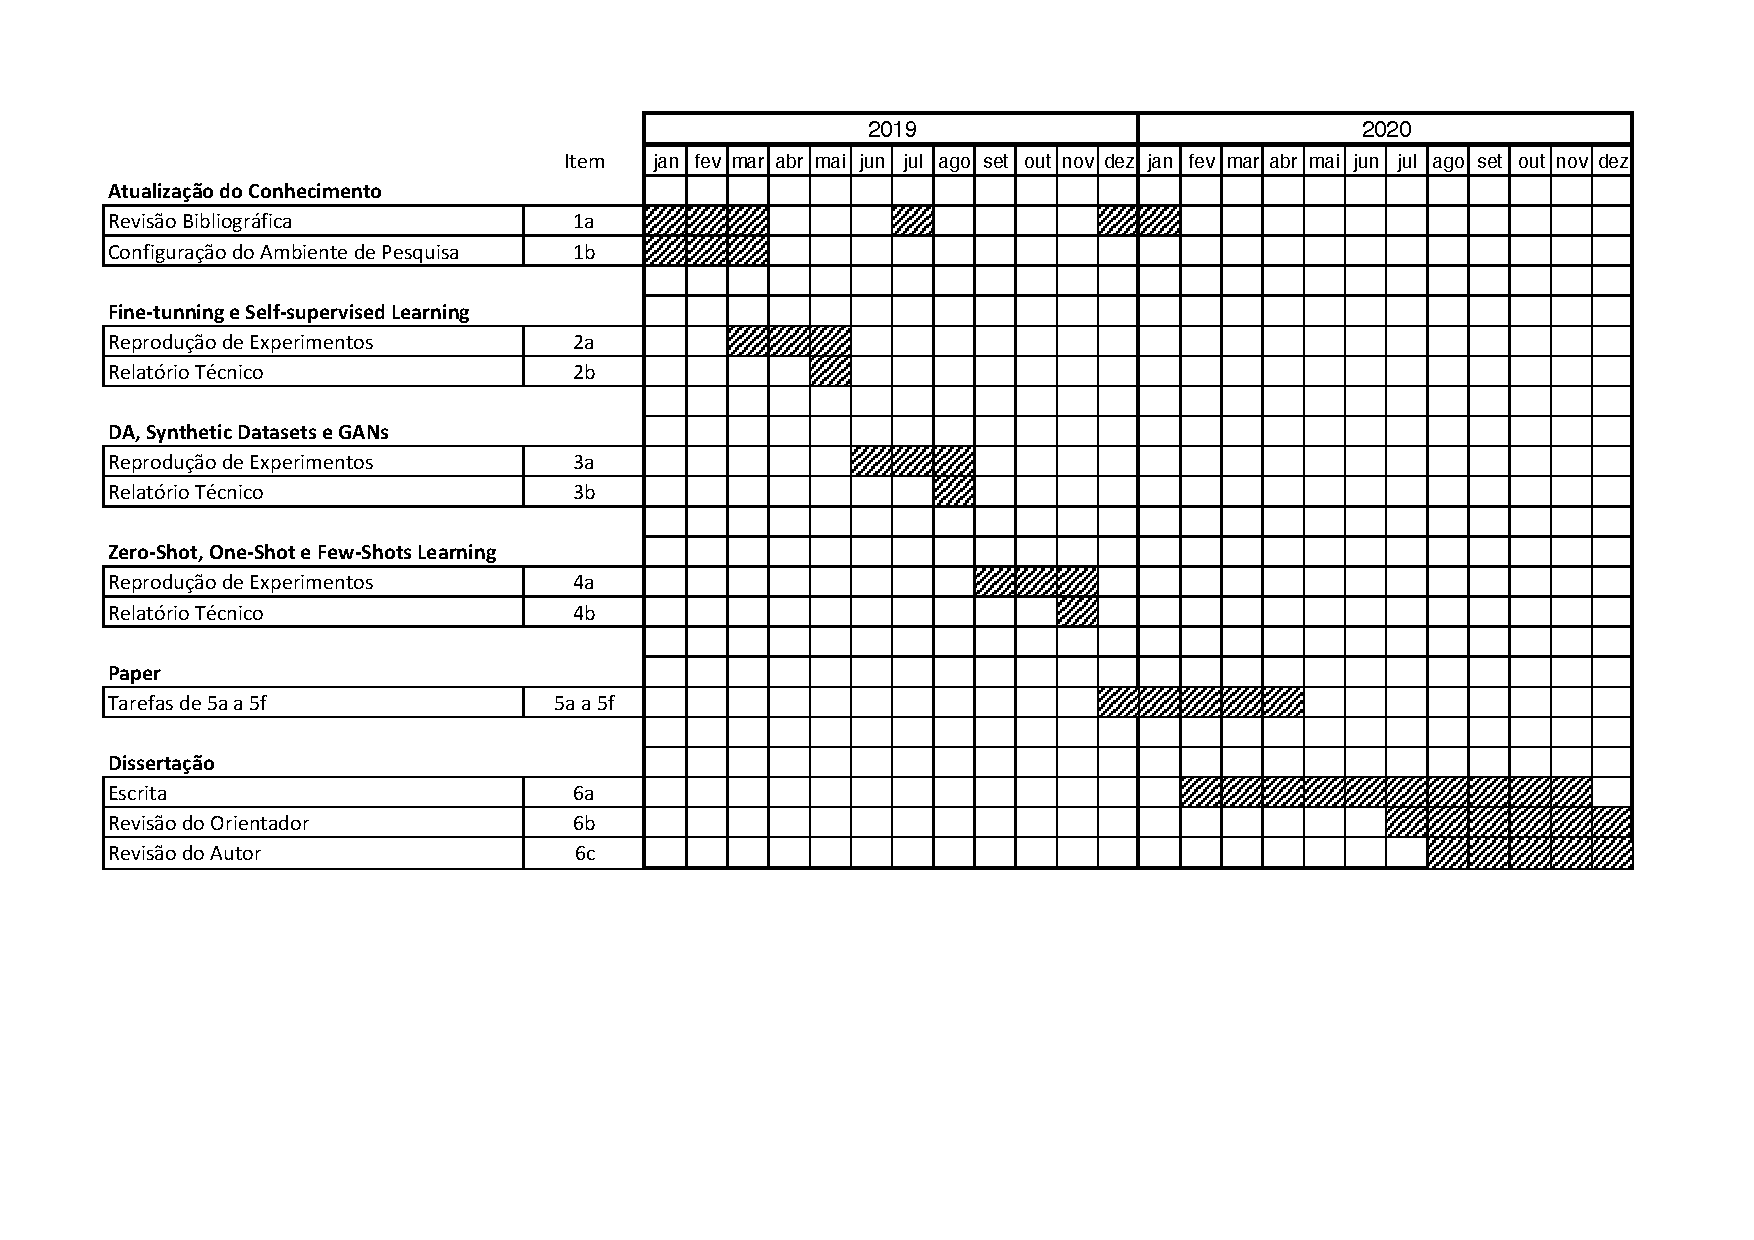
\includegraphics[
    page=1,
    width=0.8\textwidth,
    height=\textheight,
    keepaspectratio
]{gantt.pdf}
\end{center}
%
%----------------------------------------------------------------------------------------
%	BIBLIOGRAPHY
%----------------------------------------------------------------------------------------

\renewcommand{\refname}{Bibliografia} % Change the default bibliography title

\bibliography{references} % Input your bibliography file

%----------------------------------------------------------------------------------------

\end{document}